\documentclass[a4paper]{article}
\usepackage[T1]{fontenc}
\usepackage{amsmath}
\usepackage{amssymb}
\usepackage{float}
\usepackage[utf8]{inputenc}
\usepackage{graphicx}
\usepackage[italian]{babel}
\begin{document}

\author{Lorenzo Dentis, lorenzo.dentis@edu.unito.it}
\title{Esercizio 1}
\maketitle

\section{logica proposizionale}
\subsection{Esercizio 1}
Which of the following propositional formulas represents the sentence, 'He will come on the 8:15 or the 9:15 train; if the former, he will have time to visit us', where
\begin{itemize}
	\item p means 'He will come on the 8:15'
	\item q means 'He will come on the 9:15'
	\item r means 'He will have time to visit us'
\end {itemize}
Risposta 5: $(p \lor  q) \land (p \rightarrow r)$
\subsection{Esercizio 2}
Which of the following sentences has the logical form $(p \land q) \rightarrow r$ ?\\
Risposta 3: If inflation is up and an election is approaching, then public borrowing goes up.
\subsection{Esercizio 3}
Which of the following propositional formulas is satisfied by the valuation which assigns T to P, and F to q and r.\\
Risposta 2: $\lnot ( \lnot r \rightarrow ( p \land q))$
\subsection{Esercizio 4}
Which of the following propositional formulas is a tautology?\\
Risposta 5: $ (p \leftrightarrow q) \land (p \leftrightarrow \lnot q)$
\subsection{Esercizio 5}
Which of the following entailments is valid?\\
Risposta 2: $ p, \lnot p \leftrightarrow q \models \lnot q $
\subsection{Esercizio 6}
Risposta 3:
\begin{displaymath}
\begin{array}{|c c c|c|}
p & q & r & (p \rightarrow q) \lor \lnot (r \land \lnot q) \\
\hline 
T & T & T & T \\
T & T & F & T \\
T & F & T & F \\
T & F & F & T \\
F & T & T & T \\
F & T & F & T \\
F & F & T & T \\
F & F & F & T \\
\end{array}
\end{displaymath}
\subsection{Esercizio 7}
Which of the following formulas represents the sentence 'If Smith has installed central heating, then he has sold his car or he has not paid his mortage', where:
\begin{itemize}
	\item p means 'Smith has installed central heating'
	\item q means 'Smith has sold his car'
	\item r means 'Smith has paid his mortage'.
\end{itemize}
Risposta 4: $ p \rightarrow q \lor \not r $
\subsection{Esercizio 8}
Which of the following formulas represents the sentence, 'Share prices will go up, and if interest rates go up too, there will be a recession', where:
\begin{itemize}
	\item p means 'share prices will go up'
	\item q means 'interest rates will go up'
	\item r means 'there will be a recession'.
\end{itemize}
Risposta 1: $p \land q \rightarrow r $
\subsection{Esercizio 9}
Which of the following sentences could be written as $ p \lor (q \land r)$, for suitable p, q, and r ?\\
Risposta 2 : You can go swimming, or use the sauna and the shower.
\subsection{Esercizio 10}
According to the standard convention about binding priorites, the formula, $ \lnot p \rightarrow \lnot q \land r $, is implicity one of the following. Which?\\
Risposta 4: $ ( \lnot p) \rightarrow (( \lnot q) \land r) $
\subsection{Esercizio 11}
Which of the following formulas has the parse tree:\\
\begin{figure}[H]
	\centering
	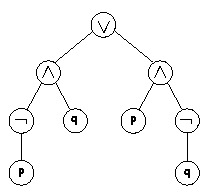
\includegraphics[scale = 0.5]{parsetree.jpg}
\end{figure}
Risposta 1: $ ( \lnot p \land q) \lor (p \land \lnot q) $

\section{notazioni e definizioni}
\subsection{notazioni}		
notazione per Naturali $ \mathbb{N} $, Interi $ \mathbb{Z} $, Reali $ \mathbb{R} $
\newline
Notazione per insiemi:
intersezione $\cap$ ,unione $\cup$, differenza $\setminus$, insieme potenza (power set) $\mathcal{P}
(A)$ , complemento $A^{C}$, Elemento contenuto in un insieme $ \in $, Sottinsieme $ \subset $ e sottinsieme stretto $ \subseteq $ ,

\subsection{definizioni}
\subsubsection{relazioni}
\begin{itemize}
	\item prodotto Cartesiano di due insiemi\\
il prodotto cartesiano di due insiemi $A$ e $B$ è l'insieme delle coppie ordinate $(a,b)$ con $a \in A$ e $b \in B$ Formalmente:\\
$A\times B:=\{(a,b):a\in A\;{\mathrm  {e}}\;b\in B\}$ 
	\item relazione binaria:\\
Si definisce relazione binaria $R$ tra due insiemi non vuoti $A$ e $B$ un sottoinsieme di $ A \times B$. Due elementi $x$ e $y$ sono messi in relazione da $R$ se: 
$(x,y)\in R\ $ ed in tal caso si scrive $xRy$.
	\item proprietà riflessiva:\\
Una relazione binaria $R$ in un insieme $X$ è detta riflessiva se ogni elemento di $X$ è in tale relazione con sé stesso.
In simboli $R$ è riflessiva se: $ \forall a\in X,\ aRa.$
	\item simmetrica:\\
una relazione binaria $R$ in un insieme$ X $è simmetrica se e solo se, presi due elementi qualsiasi $a$ e $b$, vale che se $a$ è in relazione con $b$ allora anche $b$ è in relazione con $a$.\\
In simboli: $\forall a,b\in X,\ aRb\Rightarrow bRa$
	\item transitiva:\\

	\item relazione di equivalenza:
	\item chiusura transitiva di una relazione
	\item Funzione
	\item Funzione  di arietà n,
	\item funzione iniettiva,
	\item funzione suriettiva,
	\item funzione biiettiva
\end{itemize}
\subsubsection{Stringhe e linguaggi}
\subsubsection{Grafi}
\subsubsection{Matrici}
\end{document}
